\documentclass[12pt]{article}
\usepackage[utf8]{inputenc}
\usepackage{graphicx}
\usepackage{amssymb}
\usepackage{amsthm}
\usepackage{amsmath}
\usepackage{amssymb,mathtools}
\usepackage{lipsum}
\usepackage{array}
\usepackage{wrapfig}
\usepackage{multirow}
\usepackage{tabularx}
\usepackage{graphicx}
\usepackage[a4paper,width=150mm,top=25mm,bottom=25mm,bindingoffset=6mm]{geometry}
\renewcommand{\baselinestretch}{1.2}
\usepackage[style=authoryear,sorting=nty,maxcitenames=1]{biblatex}
\addbibresource{references.bib}

\begin{document}
\begin{titlepage}
	\begin{center}
										
		\line(1,0){400}\\
		\huge{\bfseries Computational study of acoustic waves emitted by collapsing bubbles}\\
		\line(1,0){400}\\
		[3.5cm]
		\textsc{Comprehensive Exam Report}\\
		[4cm]
		Submitted by\\
		[.5cm]
		{Magu Raam Prasaad R}\\
		[2.cm]
		Department of Mechanical Engineering\\
		Indian Institute of Science\\
		Bangalore
								
	\end{center}
\end{titlepage}
\section*{Introduction}
The high-speed rotary motion of submerged propeller blades results in the formation of cavitation bubbles. These cavitation bubbles undergo significant shape variations and collapse violently. Cloud of collapsing cavitation bubbles emits blastwaves and are the source of acoustic waves. 
Accurate prediction of the sound waves emitted from interacting collapsing bubbles is of significant importance in marine hydrodynamics. 
The present work aims to carry out a large-scale numerical simulation of single and multiple cavitation bubble collapse process to develop a detailed understanding of the acoustic wave emission and propagation. 

Early investigations on the acoustic waves emitted from oscillating bubbles relied on theoretical analysis of the simplified radial dynamics (\cite{Rayleigh},\cite{Plesset}, \cite{Prosperetti}). Developments in computational power and methodologies (\cite{SHUKLA20107411}, \cite{SHUKLA2014508}, \cite{Pantano}) has enabled detailed numerical simulation of the aspherical collapse process (\cite{freund2009shock}, \cite{jamaluddin2011collapse}). However, 
numerical simulation of acoustic waves emitted by a cloud of bubbles is computationally expensive. To overcome the challenge, we use the massively parallel high-speed compressible multiphase solver developed in the lab. We use the higher-order low dissipative (WENO-ADER) scheme with interface and shock-capturing to accurately capture the propagation of underwater sound waves over long distances.
\subsection*{Objective}
\begin{enumerate}
	\item To conduct fully parallel detailed numerical simulations of cloud cavitation collapse.
    \item An efficient technique for quantification of sound waves radiated from distributions of interacting cavitation bubbles.
\end{enumerate}
\section*{Computational Approach}
\subsection*{Acoustic wave equation}
We write down the acoustic wave equation as,
\begin{equation}\label{2nd order wave}
	\frac{\partial{}^{2}{u}}{\partial{t}^{2}}- c^{2}\nabla{}^{2}{u}=0
\end{equation}  
We convert the second-order wave equation to two first order equations,
\begin{equation}\label{u update}
    \frac{\partial{u}}{\partial{t}}=v
\end{equation}
\begin{equation}\label{v update}
    \frac{\partial{v}}{\partial{t}}= c^{2}\nabla{}^{2}{u}
\end{equation}
\subsection*{Discretization}
We discretize the space into finite volume cells and enumerate the cell centers using the index $i=0,1,2,3,...,N-1$. We approximate the unknowns $u(\mathbf{x},t)$ and $v(\mathbf{x},t)$ in space by taking the volume average on each cell.
\begin{equation}
    \Bar{u}_{i} = \frac{1}{V_{i}}\int_{\Omega_{i}}u(\mathbf{x},t)d\mathbf{x} \hspace{1.4cm} i=0,1,2,3,...,N-1
\end{equation}
\begin{equation}
    \Bar{v}_{i} = \frac{1}{V_{i}}\int_{\Omega_{i}}v(\mathbf{x},t)d\mathbf{x} \hspace{1.4cm} i=0,1,2,3,...,N-1
\end{equation} 
The unknowns are written as vectors $\mathbf{u} = (\Bar{u}_{0}, \Bar{u}_{1}, ..., \Bar{u}_{N-1})$ and $\mathbf{v} = (\Bar{v}_{0}, \Bar{v}_{1}, ..., \Bar{v}_{N-1})$. We discetize the eqs \ref{u update} and \ref{v update} in space and get the following set of equations.
\begin{equation}\label{discrete u update }
    \frac{d\mathbf{u}}{dt} = \mathbf{v}
\end{equation}
\begin{equation}\label{discrete v update}
    \frac{d\mathbf{v}}{dt} = c^{2}\mathrm{L}\mathbf{u}
\end{equation}
Finally, we write down the spatially discretized equations in the following form.
\begin{gather}\label{coupled equations}
 \frac{d}{d{t}}\begin{bmatrix} \mathbf{u} \\ \mathbf{v} \end{bmatrix}
 =
  \begin{bmatrix}0 & I \\c^{2}L&0 \end{bmatrix}\begin{bmatrix} \mathbf{u} \\ \mathbf{v} \end{bmatrix}
\end{gather}
We integrate the above ODE system using the SSPRK54 scheme.
\subsection*{Reconstruction}
To compute the Laplacian operator in equation \ref{discrete v update}, we need to reconstruct the polynomial ${u}(\mathbf{x})$ from $\mathbf{u}$ vector. For each cell, we use the central WENO polynomial for reconstruction. We give an example of central 3rd order WENO polynomial reconstruction for 2d unstructured mesh (\cite{BALSARA}),
\begin{equation}\label{polynomial}
    u(x,y) = u_{o} + \phi_{x}u_{x} + \phi_{y}u_{y} + \phi_{xx}u_{xx} + \phi_{yy}u_{yy} + \phi_{xy}u_{xy}
\end{equation}
\begin{equation*}
    \phi_{x} = \frac{1}{h}(x - x_{o})
\end{equation*}
\begin{equation*}
    \phi_{y} = \frac{1}{h}(y - y_{o})
\end{equation*}
\begin{equation*}
    \phi_{xx} = \frac{1}{h^2}{(x - x_{o})}^2 - c_{1}
\end{equation*}
\begin{equation*}
    \phi_{yy} = \frac{1}{h^2}{(y - y_{o})}^2  - c_{2}
\end{equation*}
\begin{equation*}
    \phi_{yy} = \frac{1}{h^2}{(x - x_{o})}{(y - y_{o})}  - c_{3}
\end{equation*}
where $x_{o} = \frac{1}{A_{o}}\int_{o} x dA$ and $y_{o} = \frac{1}{A_{o}}\int_{o} y dA$ are coordinates of the cell center and the coefficients are defined as,
\begin{equation*}
c_{1} = \frac{1}{A_{o}}\int_{o} \frac{1}{h^2}{(x - x_{o})}^2  dA,\hspace{0.2cm} c_{2} = \frac{1}{A_{o}}\int_{o} \frac{1}{h^2}{(y - y_{o})}^2 dA \hspace{0.2cm}, \hspace{0.2cm}c_{3} = \frac{1}{h^2}(x - x_{o})(y - y_{o})
\end{equation*}
We take the volume average of the polynomial in each vertex sharing neighbor cells and equate them to $\Bar{u}_{i}$ as shown in the following equation.  
\begin{equation}
    \frac{1}{A_{i}}\int_{i}u(x,y)dA = \Bar{u}_{i} \hspace{1.4cm} i=1,2,3,...,n
\end{equation}
where, $n$ is the number of cells sharing their vertex.
This results in a Linear system of equations $\mathbf{A}\mathbf{x} = \mathbf{b}$
\begin{gather*}
   \begin{bmatrix}
   \frac{1}{A_{1}}\int_{1}\phi_{x}dA& \frac{1}{A_{1}}\int_{1}\phi_{y}dA&
   ... &
   \frac{1}{A_{1}}\int_{1}\phi_{xy}dA \\
   \frac{1}{A_{2}}\int_{2}\phi_{x}dA& \frac{1}{A_{2}}\int_{2}\phi_{y}dA&
   ... &
   \frac{1}{A_{2}}\int_{2}\phi_{xy}dA \\
   .\\
   .\\
   .\\
   \frac{1}{A_{n}}\int_{n}\phi_{x}dA& \frac{1}{A_{n}}\int_{n}\phi_{y}dA&
   ... &
   \frac{1}{A_{n}}\int_{n}\phi_{xy}dA \\
   \end{bmatrix}
   \begin{bmatrix}
   u_{x}\\
   u_{y}\\
   u_{xx}\\
   u_{yy}\\
   u_{xy}\\
   \end{bmatrix} =    \begin{bmatrix}
   \Bar{u}_{1} - \Bar{u}_{0}\\
   \Bar{u}_{2} - \Bar{u}_{0}\\
   .\\
   .\\
   .\\
   \Bar{u}_{n} - \Bar{u}_{0}\\
   \end{bmatrix}
\end{gather*}
We solve the above system for $\mathbf{x}$ that minimizes $||\mathbf{A}\mathbf{x} - \mathbf{b}||$.
\subsection*{Laplacian}
Now, we discretize the Laplacian operator for the $i$th cell,
\begin{equation}\label{Laplacian}
    \nabla{}^{2}u\Big|_{i} \approx \frac{1}{V_{i}}\int_{\Omega_{i}}\nabla{}^{2}ud\mathbf{x}
\end{equation}
We use the Gauss divergence theorem to integrate eqs \ref{Laplacian}.
\begin{align}
\frac{1}{V_{i}}\int_{\Omega_{i}}\nabla{}^{2}ud\mathbf{x} = \frac{1}{V_{i}}\sum_{f}\int_{f}\nabla{u}.\mathbf{n}ds\\
= \frac{1}{V_{i}}\sum_{f}\sum_{q}\nabla{u}.\mathbf{n}w\Big|_{q}
\end{align}
and approximate the face integral using the quadrature formula.
We evaluate the gradient of the reconstruction polynomial at the quadrature point.
\begin{equation}
    \nabla{u}_{q} = \frac{\nabla{u}_{q}^{L} + \nabla{u}_{q}^{R}}{2}
\end{equation}
\section*{Results}
\subsection*{Bubble collapse near a rigid wall}
\begin{figure}[h]
	\centering
	\begin{minipage}[b]{0.3\textwidth}
	  	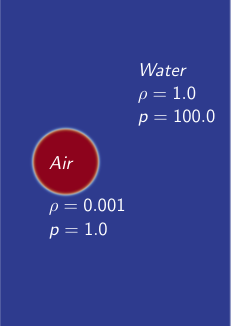
\includegraphics[width=\textwidth]{initial_bubble.png}
	  \caption{initial state}
	  \label{initial condition}
	\end{minipage}
	\hfill
	\begin{minipage}[b]{0.42\textwidth}
	  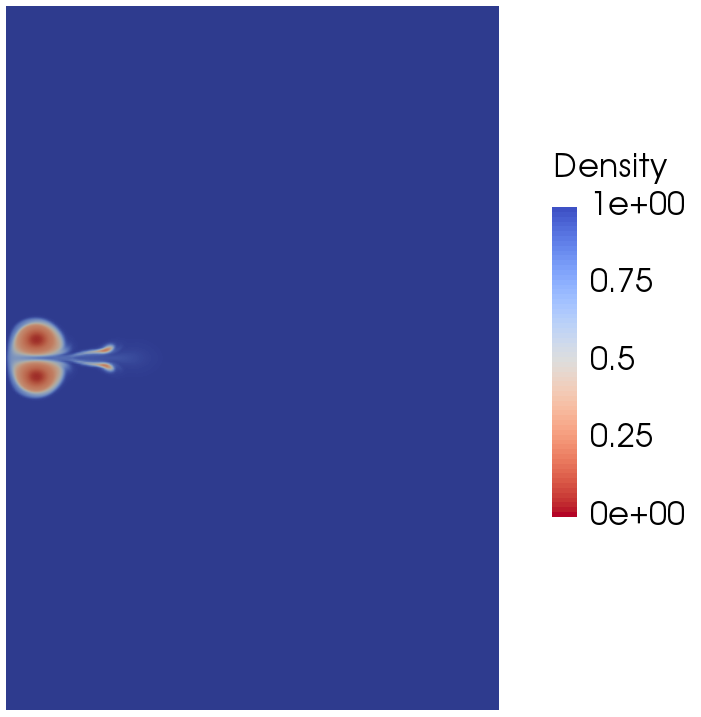
\includegraphics[width=\textwidth]{bubble_collapse.png}
	  \caption{density field at t = 1.5}
	  \label{density plot at t = 1.5}
	\end{minipage}
  \end{figure}
We test our compressible multiphase Euler equation solver by simulating a bubble collapse near a rigid wall. Our numerical setup consists of a Rectangular domain $\Omega = [-2,5]\times[-5,5]$ with an air bubble in quiescent water. We set up the initial density and pressure of the bubble and fluid, as shown in figure \ref{initial condition}. Both the bubble and surrounding fluid are at rest initially. The domain is discretized using structured grid $350 \times 500$. The boundary conditions are reflective for the left wall, and other boundaries are transmissive. The pressure difference between the bubble and the surrounding fluid initiates the bubble collapse process, and the bubble travels further towards the left wall and collapses near the wall (see figure \ref{density plot at t = 1.5}).  
\subsection*{Standing wave solution}
We solve the acoustic wave equation on a 2d square domain $\Omega = [-1,1]\times[-1,1]$. We enforce the homogeneous Dirichlet boundary condition with the initial condition $u = sin(k_{x}x)sin(k_{y}y)$ and
${\partial u}/{\partial t} = 0$, where $k_{x} = {2\pi}$, $k_{y} = {2\pi}$, $\omega = \sqrt{8}\pi$. We employ structured grid discretization with the fourth-order central WENO polynomial in space and the SSPRK54 scheme in time. We did spatial convergence study and get fourth-order convergence in space as shown in table \ref{table:1} for the standing wave solution $u(\mathbf{x},t) = cos(\omega t)sin(k_{x}x)sin(k_{y}y)$.
\begin{table}[h]
	\centering
	\begin{tabular}{ |c|c|c|c|c| }
		\hline
		N   & $L_{\infty}$norm & $L_{2}$ norm & $L_{2}$ rate & $L_{\infty}$ rate \\ 
		\hline
		32  & 1.60e-03         & 8.32e-04     & -            & -                 \\
		64  & 1.06e-04         & 5.35e-05     & 3.95         & 3.91              \\
		128 & 6.73e-06         & 3.37e-06     & 3.98         & 3.97              \\
		256 & 4.22e-07         & 2.11e-07     & 3.99         & 3.99              \\
		\hline
	\end{tabular}
	\caption{Convergence table for standing wave solution}
	\label{table:1}
\end{table}
\subsection*{Plane wave solution}
We solve the acoustic wave equation on a 2d unstructured periodic grid. We perturb the domain using sinusoidal deformation function $x = X + 0.3sin\Big(\frac{\pi Y}{2}\Big)$ and $y = Y + 0.4sin\Big(\frac{\pi X}{2}\Big)$ as shown in figure \ref{grid}. Where $(X,Y) \in [-2,2] \times [-2,2] $ are the coordinates of structured grid vertices and $(x,y)$ are the coordinates of deformed grid vertices. We set the initial condition $u = sin(k_{x}x + k_{y}y)$ and
$\frac{\partial u}{\partial t} = -\omega cos(k_{x}x + k_{y}y)$,
where $k_{x} = {\pi}/{2}$, $k_{y} = {\pi}/{2}$, $\omega = 2\pi$ (see figure \ref{plane wave}) for the plane wave solution $u(\mathbf{x},t)=sin(k_{x}x + k_{y}y - \omega t)$. We did spatial convergence study and get fourth-order convergence as show in \ref{table:2}. 
\begin{figure}[h!]
	\centering
	\begin{minipage}[b]{0.34\textwidth}
	  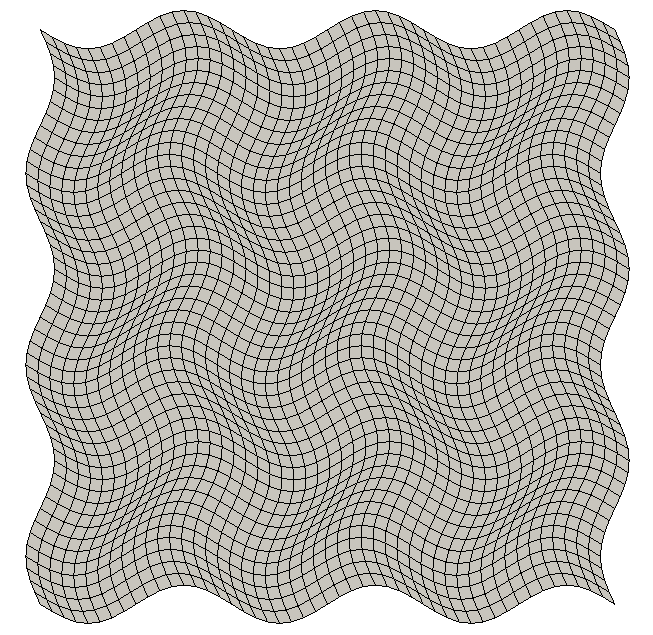
\includegraphics[width=\textwidth]{grid.png}
	  \caption{perturbed grid}
	  \label{grid}
	\end{minipage}
	\hfill
	\begin{minipage}[b]{0.45\textwidth}
	  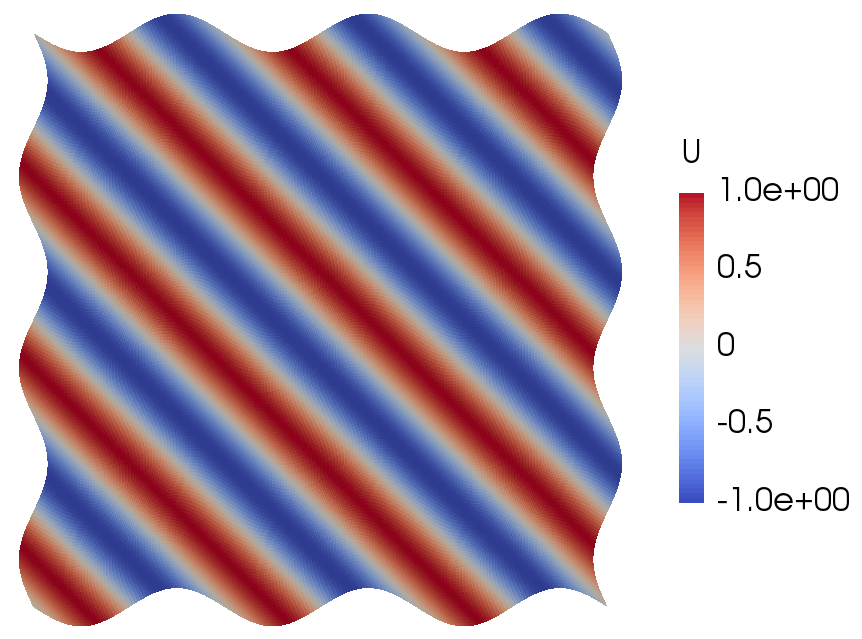
\includegraphics[width=\textwidth]{plane_wave_initial.png}
	  \caption{initial condition}
	  \label{plane wave}
	\end{minipage}
  \end{figure}
  \begin{table}[h!]
	  \centering
	  \begin{tabular}{ |c|c|c|c|c| } 
		\hline
		N   & $L_{\infty}$norm & $L_{2}$ norm & $L_{2}$ rate & $L_{\infty}$ rate \\ 
		\hline
		32  & 1.12e-03         & 4.14e-04     & -            & -                 \\
		64  & 7.93e-05         & 2.92e-05     & 3.82         & 3.82              \\
		128 & 5.10e-06         & 1.88e-06     & 3.95         & 3.95              \\
		256 & 3.21e-07         & 1.18e-07     & 3.98         & 3.98              \\
		\hline
	\end{tabular}
	\caption{Convergence table for plane wave solution}
	\label{table:2}
  \end{table}
\section*{Conclusion}
\begin{enumerate}
	\item Simulated collapsing bubble using higher order fully parallel WENO based compressible multiphase flow solver developed in the lab.
	\item Solved acoustic wave equation in 2d structured and unstructured grid using WENO4 SSPRK54 scheme.
\end{enumerate}
\subsection*{Future work}
\begin{enumerate}
	\item To carry out large scale simulation of single and multiple cavitation bubble collapse.
	\item To carry out detailed analysis of acoustic waves emitted in the collapse process. 

\end{enumerate}
\printbibliography
\end{document}